\documentclass{powerdot}

\pdsetup{lf={Jordan Thayer (Draper)},
	 rf={15 Puzzle}}

% for including postscript
\usepackage{graphicx}
\usepackage{amsmath}
\usepackage{latexsym} %%box def
\usepackage{pstricks,,pst-node,pst-tree}
\usepackage{amssymb}
\DeclareMathOperator*{\argmin}{argmin}
% get my macros

% shorthand for including the figures
\newcommand{\figwidth}[1]{%
	\bc
	\includegraphics[width=\textwidth]{#1}
	\ec
}
\newcommand{\figheight}[1]{%
	\bc
	% height=2.8in
	\includegraphics[height=2.8in]{#1}
	\ec}

\newcommand{\qspace}{\vspace{0.1in}}
\newcommand{\myred}[1]{{\color{red} #1}}
\newcommand{\mygreen}[1]{{\color{green} #1}}
\newcommand{\myyellow}[1]{{\color{yellow} #1}}
\newcommand{\turnred}[1]{{\onslide*{1}{#1}\onslide*{2}{\color{red} #1}}}
\newcommand{\myblue}[1]{{\color{blue} #1}}

\newcommand{\mybf}[1]{\textcolor{red}{\bf #1}}
\newcommand{\myem}[1]{\textcolor{blue}{\em #1}}
\newcommand{\openfH}{{\myit open}_{\widehat{f}}}
\newcommand{\openf}{{\myit open}_f}


\title{AI For Games: What Are We Talking About?}
\author{Jordan Thayer}

\date{\vspace{0.2in}}
\begin{document}
\maketitle

\section[slide=false]{Logistics}
\begin{slide}{Syllabus}
  \begin{enumerate}
    \item Introduction To Games
      \subitem Syllabus
      \subitem Types of Games
      \subitem Terminology
      \subitem Brief History of Games and AI
    \item Minimax Tree Search
    \item $\alpha$-$\beta$ pruning
    \item Multi-Armed Bandits and Monte Carlo Tree Search
    \item Implementing Monte Carlo Tree Search
    \item Weak and Strong Solutions to Games, Checkers
  \end{enumerate}
\end{slide}

\begin{slide}{Today\hfill Introduction to Games}
  \begin{itemize}
    \item Types of Games
    \item Terminology
    \item Brief History of AI and Games
  \end{itemize}
\end{slide}
%%%%%%%%%%%%%%%%%%%%%%%%%%%%%%%%%%%%%%%%%%%%%%%%%%%%%%%%%%%%%%%%%%%
\section{Types of Games}

\begin{slide}{Single Player Games}
  \twocolumn{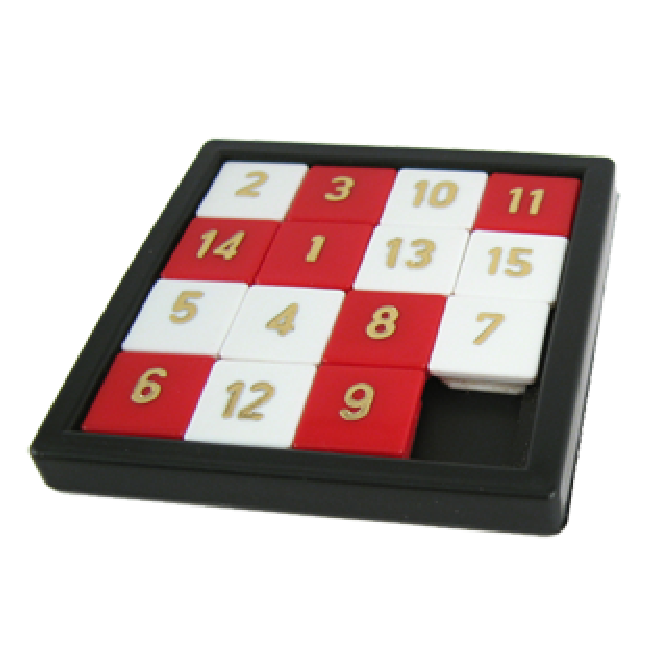
\includegraphics[width=2in]{images/15puz.eps}}
            {
              \vspace{1.5in}
              \begin{itemize}
              \item Puzzley
              \item No antagonist (other than the environment)
              \end{itemize}
            }
\end{slide}

\begin{slide}{Two Player Games}
  \twocolumn{
    \includegraphics[width=2in]{images/Start_position_in_a_chess_game.eps}
    %% Picture of Chess
  }
            {\vspace{1.5in}
              \begin{itemize}
                \item Exactly two players
                \item Usually played in turns
                \item Typically Zero-sum
              \end{itemize}
            }
\end{slide}

\begin{slide}{N-Player Games}
  \twocolumn{
    %% Picture of Catan
    \includegraphics[width=2in]{images/Sample-Setup.eps}
  }
            {\vspace{1.5in}
              \begin{itemize}
                \item More Than Two Players
                \item Produces a ranking of players
                \item Coallitions form and disolve during play
              \end{itemize}
            }
\end{slide}

\begin{slide}{Games with Chance}
  \twocolumn{
    %% Picture of Backgammon
    \includegraphics[width=2in]{images/Backgammon_lg.eps}
  }
  {\begin{itemize}
      \item Dice
      \item Spinners
      \item Shuffling
    \end{itemize}
    }
\end{slide}

\begin{slide}{Games with Imperfect Information}
  \twocolumn{
    %% Picture of Statego
    \includegraphics[width=3in]{images/800px-stratego_board.eps}
  }
            {\vspace{2in}
              \begin{itemize}
                \item Flipping Tiles, Cards
                \item ``Hands''
                \item Asymmetric Information
            \end{itemize}}
\end{slide}

\begin{slide}{Taxonomy of Games and Approaches}
  Games:
  \begin{tabular}{lll}
               & Perfect Information & Imperfect Information \\
    One Player & Permutation Puzzles & Solitaire \\
    Two Player & Chess, Checkers     & Stratego \\
    N Players  & Some Board Games    & Most Card Games \\
  \end{tabular}
  \vspace{0.5in}
  Approaches:
  \begin{tabular}{lll}
               & Perfect Information & Imperfect Information \\
    One Player & Depth First Search & Policy Search \\
    Two Player & Game Tree Search   & MDP \& POMDP Solvers \\
    N Players  & Game Tree Search   & Regret Minimization \\
  \end{tabular}
\end{slide}

%%%%%%%%%%%%%%%%%%%%%%%%%%%%%%%%%%%%%%%%%%%%%%%%%%%%%%%%%%%%%%%%%%%
\section{Two Player Perfect Information Games}

\begin{slide}{Two Player Perfect Information Games}
  \begin{itemize}
    \item Exactly Two Players
    \item All actions are deterministic
    \item Shared game representation
    \item Each game is self contained
  \end{itemize}
\end{slide}

\begin{slide}{Turns and Ply}
  %% Draw an initial game state
  \onslide*{1}{\includegraphics[height=3in]{images/blank_board.eps}}
  %% Draw player 1s move
  \onslide*{2}{\includegraphics[height=3in]{images/ply_1_5.eps}}
  %% Add player twos move
  \onslide*{3}{\includegraphics[height=3in]{images/ply_2_1.eps}}
\end{slide}

\begin{slide}{Tree Search}
  %% Draw the inital game state again
  \onslide*{1}{\includegraphics[height=3in]{images/blank_board.eps}}
  %% Show each possible first move, setting up a tree of depth 1
  \onslide*{2}{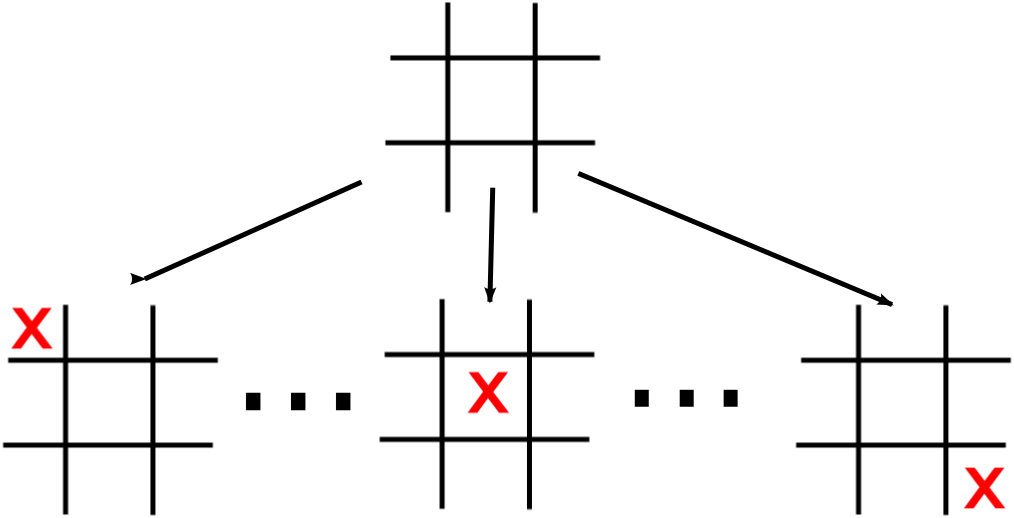
\includegraphics[width=3in]{images/one_ply.eps}}
  %% Show each possible response, shwoing a tree of depth 2
  \onslide*{3}{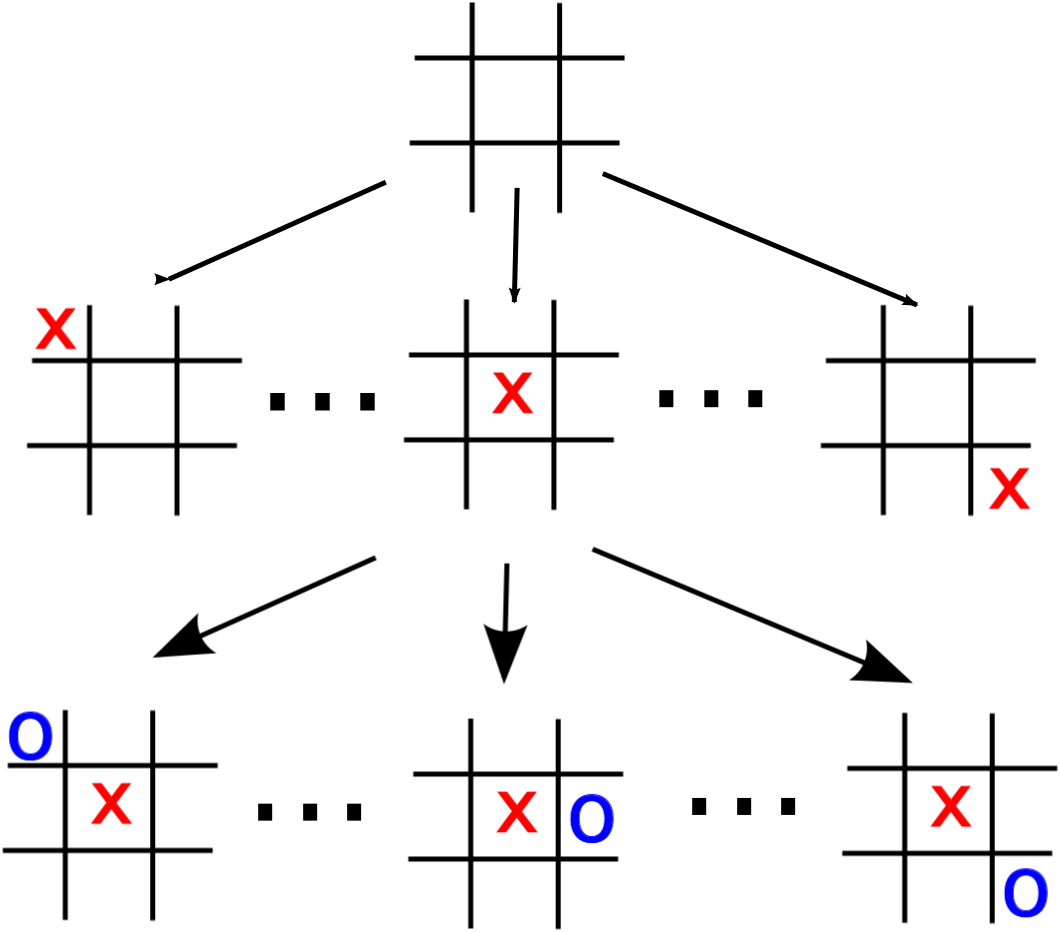
\includegraphics[width=3in]{images/two_ply.eps}}
\end{slide}

\begin{slide}{Graph Search}
  %% Show another ply, inducing a DAG
  %% Draw the inital game state again
  \onslide*{1}{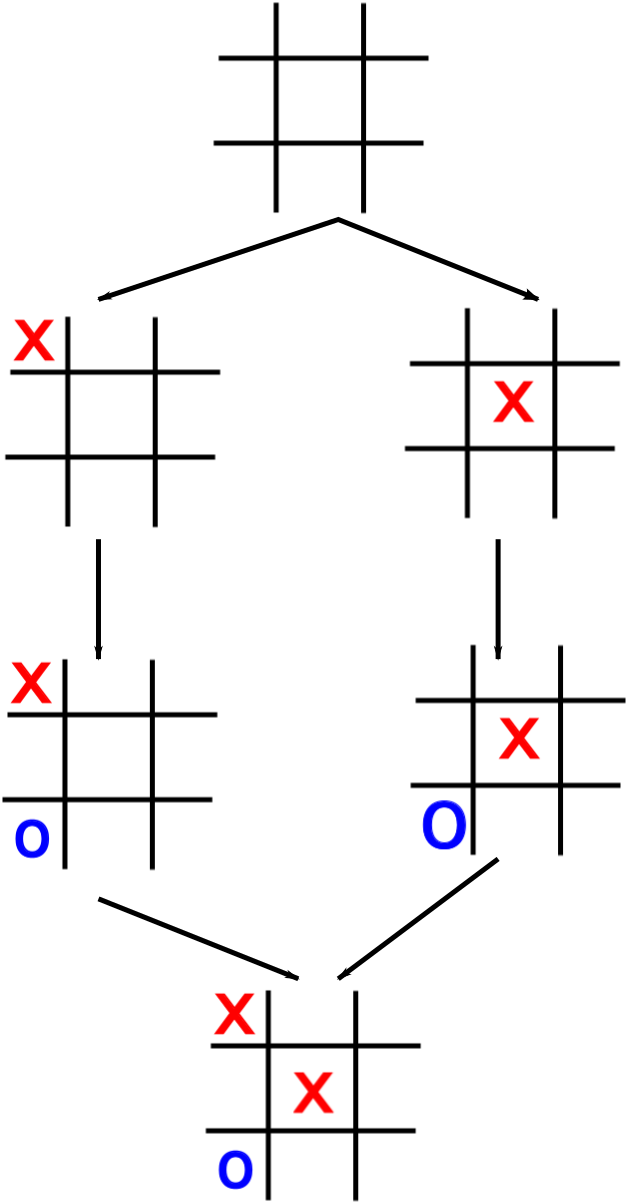
\includegraphics[height=3in]{images/graph_ex.eps}}
\end{slide}

\begin{slide}{Solutions, Strategies}
  \begin{description}
    \item[Ultra-Weak] Show whether player one wins, loses, or draws given
      perfect play on both sides.
    \item[Weak] Provide an algorithm that secures a win for one player, or a
      draw for either givenany possible move from the opposing player.
    \item[Strong] Provide an algorithm that can play perfectly from
      arbitrary, but legal, board positions.
  \end{description}
\end{slide}

%%%%%%%%%%%%%%%%%%%%%%%%%%%%%%%%%%%%%%%%%%%%%%%%%%%%%%%%%%%%%%%%%%%
\section{AI and Games}

\begin{slide}{McCarthy Studies Chess Players}
  1956 - John McCarthy conference on Artificial Intelligence\\
  1959 - Kotok, first program to play chess written by McCarthy\\
  1978 - Several automated players (Belle, Chess4.7) start beating masters\\\
  1989 - Kasparov Competes against Deep Thought (And wins)\\
  1996 - Deep Blue Beats Kasparov for one game, but loses tournament\\
  2003 - Junior Ties Kasparov\\
  2005 - Hydra (Custom hardware) wins 5.5 - 0.5 against grand master\\
  2009 - Commodity hardware performs at grand master levels\\
\end{slide}

\begin{slide}{Checkers and the March to Chinook}
  1951 - Starchey writes the first AI for checkers \\
  1959 - Samuel Publishes "Some Studies in Machine Learning Using the game of Checkers", invents alpha-beta pruning\\
  1989 - Schaeffer makes Chinook\\
  1994 - Chinook beats the world human champion Lafferty\\
  2003 - Chinook completes its 10 piece database with 5 pieces on each side.\\
  2004 - The Chinook team announces that the tournament opening in English draughts called the White Doctor (10–14 22–18 12–16) is proven to be a draw.\\
  2007 - The journal Science publishes Schaeffer's team's article "Checkers Is Solved", presenting their proof that the best a player playing against Chinook can achieve is a draw.
\end{slide}

\begin{slide}{Go}
  1968 - Zorbist studies go and pattern recognition in his thesis \\
  1981 - Go players for home computers are available, and awful\\
  1987 - Monte Carlo Tree Search applied to games, no one takes it seriously\\
  1992 - MCTS used in Go for the first time\\
  1998 - Go Intellect loses to children with a 25-30 stone handicap\\
  2006 - Upper Confidence Bounds for Trees published, used in MoGo\\
  2008 - MoGo is Dan in 9x9 go\\
  2012 - Zen wins 3:1 on a 19x19 board\\
  2015 - Alpha Go wins without a handicap against professional players\\
  2016 - Alpha Go beats a 9-dan player
\end{slide}

\begin{slide}{Other Victories}
Backgammon (1979)\\
Connect 4 (Solved in 1988)\\
Othello (Solved 1993)\\
Mancala (Solved 2002)\\
Rock Paper Scissors\\
Crosswords (2006)\\
Hold'em (weakly solved in 2015)
\end{slide}

\begin{slide}{Syllabus}
  \begin{enumerate}
    \item Introduction To Games
      \subitem Syllabus
      \subitem Types of Games
      \subitem Terminology
      \subitem Brief History of Games and AI
    \item Minimax Tree Search
    \item $\alpha$-$\beta$ pruning
    \item Multi-Armed Bandits and Monte Carlo Tree Search
    \item Implementing Monte Carlo Tree Search
    \item Weak and Strong Solutions to Games, Checkers
  \end{enumerate}
\end{slide}

\end{document}
